\documentclass{standalone}
\usepackage{tikz}
\begin{document}

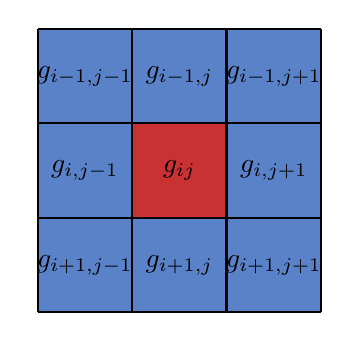
\begin{tikzpicture}[scale=1.2]

% Colors
\definecolor{cellblue}{RGB}{90,130,200}
\definecolor{cellred}{RGB}{200,50,50}

% Draw cells
\foreach \x in {0,1,2} {
  \foreach \y in {0,1,2} {
    \fill[cellblue] (\x,\y) rectangle ++(1,1);
  }
}

% Center cell
\fill[cellred] (1,1) rectangle ++(1,1);

% Grid lines
\draw[thick] (0,0) grid (3,3);

% Labels
\node at (0.5,2.5) {$g_{i-1,j-1}$};
\node at (1.5,2.5) {$g_{i-1,j}$};
\node at (2.5,2.5) {$g_{i-1,j+1}$};

\node at (0.5,1.5) {$g_{i,j-1}$};
\node at (1.5,1.5) {$g_{ij}$};
\node at (2.5,1.5) {$g_{i,j+1}$};

\node at (0.5,0.5) {$g_{i+1,j-1}$};
\node at (1.5,0.5) {$g_{i+1,j}$};
\node at (2.5,0.5) {$g_{i+1,j+1}$};

\end{tikzpicture}

\end{document}
